\documentclass[conference]{IEEEtran}
\usepackage[T1]{fontenc}
\usepackage{amsmath,amssymb}
\usepackage{graphicx}
\usepackage{xcolor}
\usepackage{tikz}
\usetikzlibrary{shapes.geometric,arrows.meta,positioning,fit}
\usepackage{booktabs}
\usepackage{url}
\newcommand{\code}[1]{\texttt{#1}}

\begin{document}

\title{Evaluating Lightweight Grid-Based Vehicle Classification and Counting
Using Resolution Sensitivity Analysis and Sequential--Parallel Benchmarking}

\author{
\IEEEauthorblockN{Jay Suriya R}
\IEEEauthorblockA{Department of Computer Science and Engineering\\
Indian Institute of Information Technology Sri City\\
Sri City, India\\
jaysuriya.r24@iiits.in}
\and
\IEEEauthorblockN{Manipriya Sankaranarayanan}
\IEEEauthorblockA{Department of Computer Science and Engineering\\
Indian Institute of Information Technology Sri City\\
Sri City, India\\
manipriya.s@iiits.in}
}

\maketitle

\begin{abstract}
Grid-based (``virtual lattice'') motion detection processes traffic video
on commodity CPUs without training, but the published lattice detector
stops at a binary occupancy grid and reports no accuracy. We extend its
front end with geometric vehicle classification, tracking and
line-crossing counting (plus density estimation and a speed estimator
whose accuracy is not evaluated) in a sequential and a two-lane parallel
Python implementation, and study the pipeline experimentally on UA-DETRAC.
A cross-implementation check found two preprocessing divergences; after
fixing them, both implementations give identical results on 12 benchmark
videos. A four-workload benchmark on a 4-core/8-thread CPU separates lane
count from threading: the thread pools slowed the same two-lane workload
(time ratio $0.860\pm0.077$, slower on all 12 videos), and the
$1.26\times$ higher ROI-frame throughput of the two-lane implementation
comes from sharing decoding and preprocessing between lanes. A
grid-resolution study with site-grouped cross-validation, counting ground
truth derived from annotated trajectories and 44 videos from unseen sites
shows that, once thresholds are re-tuned per grid, no resolution changes
macro-F1 significantly, whereas $10{\times}12$ raises the per-video count
error from 16.0 to 23.1 vehicles (Holm-adjusted $p=0.010$). The tuned
classifier exceeds an always-Car baseline in macro-F1 but not in
weighted-F1, and the counter registers only downward crossings, so it
misses 44\% of the test crossings, most of them in Lane~2.
\end{abstract}

\begin{IEEEkeywords}
vehicle classification, multi-object tracking, vehicle counting,
parallel computing, thread pool, Python GIL, benchmarking, UA-DETRAC
\end{IEEEkeywords}

\section{Introduction}
\label{sec:intro}
Existing road cameras can support vision-based vehicle counting and
classification without inductive loops or radar \cite{crouzil2016}.
Recent systems combine learned detectors with multi-object trackers,
e.g.\ YOLOv7 with DeepSORT \cite{lian2025} or an improved YOLOv8 with
BoT-SORT \cite{liu2025}; model size, power and throughput are recognized
obstacles on edge hardware \cite{zhai2023}, which lightweight
architectures and quantization reduce \cite{chang2025,macko2025}.
Classical foreground-segmentation pipelines remain a training-free
alternative for counting and coarse classification \cite{unzueta2012},
although illumination changes, shadows and occlusion make them fragile
\cite{abbas2021,chen2020}.

Two-Tier Parallel Virtual Lattice Layers (TPL2) \cite{baseline} divides
each lane's ROI into a grid, marks cells by histogram-equalized frame
differencing and per-cell contour detection, and dispatches cells and
lanes to a \code{ThreadPoolExecutor}. The TPL2 paper describes a
lattice-run counting heuristic and count-based density, leaves speed
estimation to future work, and reports execution time and memory
(26.55\% efficiency gain, 3.72\% more memory) but no accuracy metrics
\cite{baseline,muthuraja2026}. Its released code, which we build on,
stops at the occupancy grid and creates a new thread pool every frame
without persistent per-lane state (Table~\ref{tab:baseline}).

This paper is an experimental study of such a lightweight grid-based
pipeline rather than a proposal of a state-of-the-art classifier. We
contribute: (1) a classification, tracking, counting and
adaptive-density layer on that front end, implemented identically in a
sequential (\code{seq.py}) and a two-lane parallel
(\code{rparallel\_he3.py}) implementation, plus a calibration-based speed
estimator that is implemented but not validated; (2) a parallel design
with persistent pools, per-lane \code{LaneTracker} state and a
compute/draw split; (3) a cross-implementation check that found and fixed
two preprocessing divergences; (4) a four-workload benchmark that
separates the effect of processing two lanes from the effect of
threading; and (5) a grid-resolution study with site-grouped
cross-validation, trajectory-based counting ground truth, paired
statistical tests and an unseen-site test set.

\begin{table}[t]
\centering
\caption{Baseline \cite{baseline} vs.\ this paper.}
\label{tab:baseline}
\scriptsize
\setlength{\tabcolsep}{3pt}
\begin{tabular}{p{3.85cm}p{4.2cm}}
\toprule
\textbf{Baseline (paper / released code)} & \textbf{This paper} \\
\midrule
ROI grid; HE frame differencing; per-cell contours & reused; retuned parameters; two divergences fixed \\
-- & geometric vehicle classification \\
lattice-run count heuristic (paper) & tracking, duplicate suppression, line-crossing counts \\
speed left to future work & displacement-gated speed estimation \\
raw occupancy (code), count-based density (paper) & adaptive thresholds with flow blending \\
pool created per frame, no per-lane state & persistent pools, per-lane \code{LaneTracker} \\
time and memory only & UA-DETRAC accuracy; four-workload timing \\
\bottomrule
\end{tabular}
\end{table}

\section{Related Work}
\label{sec:related}
Frame differencing and background subtraction remain competitive with
more elaborate background models in urban traffic video at a fraction of
the cost \cite{cheung2004}, and support real-time counting and
classification \cite{unzueta2012,crouzil2016}. A contemporaneous
extension of the same baseline \cite{muthuraja2026} adds scene-adaptive
preprocessing (illumination classes, CLAHE, a Dark Channel Prior fog
index) and reaches 71.03\% micro-averaged F1 on 60 UA-DETRAC sequences
with Hungarian matching; its multi-\emph{process} engine reaches
$1.34\times$ over sequential execution, with inter-process serialization
and sequential tracking identified as the binding constraints. That
pipeline differs from ours, so its process-level result and our
thread-level result are not directly comparable. SORT \cite{bewley2016} and DeepSORT \cite{wojke2017}
are standard tracking alternatives to our greedy association.
Pixel-displacement speeds need a metric scale and validation against
measured speeds \cite{kamil2024}, and unstable trajectories degrade them
\cite{sangsuwan2024}. Contours follow Suzuki and Abe's border following
\cite{suzuki1985}; data come from UA-DETRAC \cite{wen2020}. CPython's GIL
serializes bytecode across threads \cite{pythongil}, but
\code{ThreadPoolExecutor} \cite{pythonfutures} can overlap native calls
that release it. Amdahl's law \cite{amdahl1967,alhayanni2020},
\begin{equation}
S(N)=\frac{1}{(1-p)+p/N},
\label{eq:amdahl}
\end{equation}
bounds the speedup for parallel fraction $p$ on $N$ workers; a
single-fraction model cannot capture contention between resources
\cite{poolla2023}. We follow reporting recommendations for reliable
benchmarking \cite{beyer2019,kalibera2013}.

\section{Methodology}
\label{sec:method}

\subsection{Pipeline Overview}
Fig.~\ref{fig:roi} shows the two ROIs and Fig.~\ref{fig:pipeline} the
per-ROI pipeline. The sequential implementation (\code{seq.py})
processes ROI~1; the two-lane parallel implementation processes ROI~1 and
ROI~2 as independent lanes. Fig.~\ref{fig:stages}
shows the intermediate results of one frame.

\begin{figure}[t]
\centering
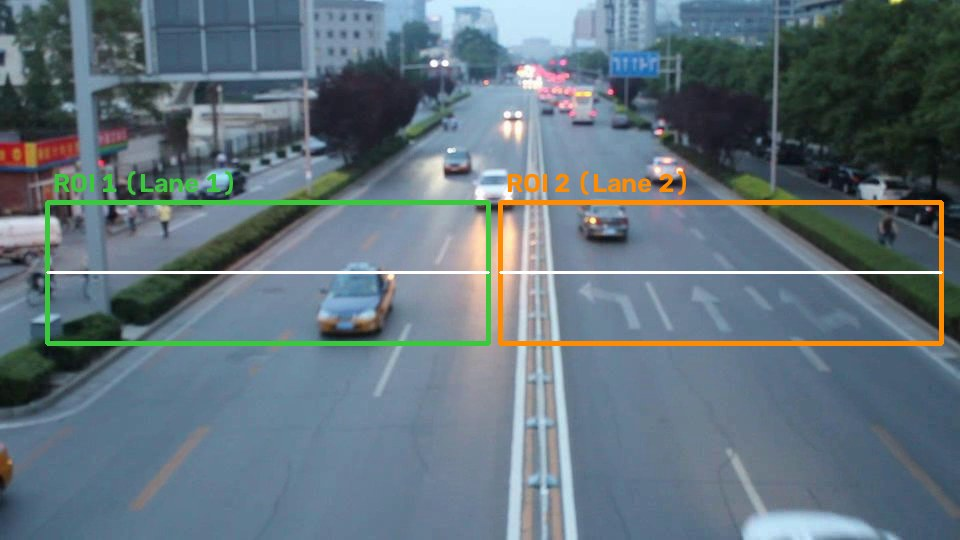
\includegraphics[width=\columnwidth]{figures/fig_roi_frame.jpg}
\caption{UA-DETRAC frame (MVI\_39761) with ROI~1 (green, Lane~1) and
ROI~2 (orange, Lane~2); white lines are the count lines.}
\label{fig:roi}
\end{figure}

\begin{figure*}[t]
\centering
\resizebox{\textwidth}{!}{%
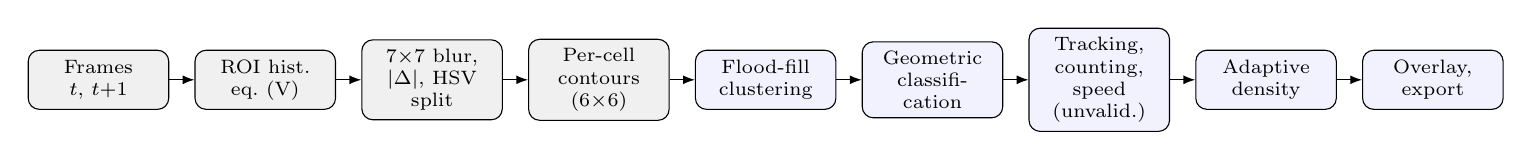
\begin{tikzpicture}[
  box/.style={draw, rounded corners, align=center, minimum height=0.75cm,
              text width=1.55cm, font=\scriptsize, fill=blue!5},
  base/.style={box, fill=gray!12},
  arr/.style={-{Latex[length=1.5mm]}}, node distance=3.2mm]
\node[base] (a) {Frames $t$, $t{+}1$};
\node[base, right=of a] (b) {ROI hist.\ eq.\ (V)};
\node[base, right=of b] (c) {$7{\times}7$ blur, $|\Delta|$, HSV split};
\node[base, right=of c] (d) {Per-cell contours ($6{\times}6$)};
\node[box, right=of d] (e) {Flood-fill clustering};
\node[box, right=of e] (f) {Geometric classification};
\node[box, right=of f] (g) {Tracking, counting, speed (unvalid.)};
\node[box, right=of g] (h) {Adaptive density};
\node[box, right=of h] (i) {Overlay, export};
\foreach \x/\y in {a/b,b/c,c/d,d/e,e/f,f/g,g/h,h/i} \draw[arr] (\x) -- (\y);
\end{tikzpicture}%
}
\caption{Per-ROI pipeline. Gray: baseline front end (reused, retuned);
blue: added in this work.}
\label{fig:pipeline}
\end{figure*}

\begin{figure*}[t]
\centering
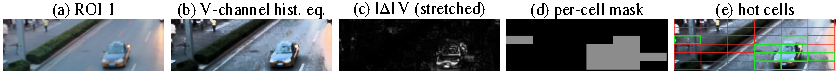
\includegraphics[width=\textwidth]{figures/fig_stages.pdf}
\caption{Processing stages for ROI~1 (MVI\_39761, frame 700): (a) input,
(b) V-channel histogram equalization, (c) absolute difference of the
blurred frames, V channel (contrast-stretched for display), (d) per-cell
thresholded and dilated masks, (e) cells with a valid contour (green).}
\label{fig:stages}
\end{figure*}

\subsection{Grid-Based Motion Detection (Baseline Front End)}
\label{sec:motion}
Both frames are histogram-equalized on the ROI's V channel (the
equalization channel is fixed to V), blurred with a $7\times7$ Gaussian
and differenced; the difference is converted to HSV and the configured
channel (V) is split out. Each cell is blurred ($5\times5$, $\sigma{=}1$),
thresholded at 60, dilated with a (cell width, cell height/2) rectangle
for 5 iterations, and marked ``hot'' if \code{cv2.findContours}
(\code{RETR\_EXTERNAL}) returns a contour larger than 100\,px$^2$ (AND
across channels if several are selected). Relative to the baseline we
retuned the threshold ($20\to60$), dilation (fixed kernel, 3
iterations $\to$ cell-sized, 5), retrieval mode (\code{RETR\_TREE} $\to$
\code{RETR\_EXTERNAL}) and blur $\sigma$ ($0\to1$), because the classifier
depends on precise cluster spans. Table~\ref{tab:params} lists all
constants.

\begin{table}[t]
\centering
\caption{Pipeline parameters (identical in both implementations).}
\label{tab:params}
\scriptsize
\setlength{\tabcolsep}{3pt}
\begin{tabular}{ll}
\toprule
ROI 1 / ROI 2 $(x,y,w,h)$ & (47,202,441,141) / (500,202,441,141) \\
Grid; cell blur / threshold & $6\times6$; $5\times5$ Gaussian / 60 \\
Dilation; min.\ contour area & (cell$_w$, cell$_h$/2), 5 iters; 100 px$^2$ \\
Track match radius; dup.\ IoU & ROI height/2; 0.40 \\
Crossing cooldown; eviction & 30 frames, 60 px; unseen $>2$\,s \\
Label EWA $\alpha$; min.\ frames scored & 0.15; 5 \\
Speed gate; smoothing & 3$\times$cell height; last 15 samples \\
Density blend; flow norm. & 0.7/0.3; 8 crossings per 2\,s \\
Density thresholds & 0.30/0.60, then 0.25/0.55 $\pm$0.10 adaptive \\
\code{\_CELL\_POOL} / \code{\_LANE\_POOL} & $\min(32,4{\times}\text{cpu})$ = 32 / 2 \\
\bottomrule
\end{tabular}
\end{table}

\subsection{Clustering and Classification}
\label{sec:classify}
Hot cells are grouped into objects by 4-connected flood fill; each
cluster gets a bounding box, centroid and the number of distinct columns
and rows it spans. With spans normalized by the grid size, a cluster is
a \textbf{Bus} if its column span exceeds 0.75 or both spans exceed
0.55, a \textbf{Van} if its row span exceeds 0.45, and a \textbf{Car}
otherwise. No appearance features are used, so the thresholds are tied
to this camera geometry. Their dependence on the lattice resolution is
examined in Section~\ref{sec:grid-sensitivity}.

\subsection{Tracking, Counting and Density}
\label{sec:tracking}
Objects are greedily matched to tracks by nearest centroid within half
the ROI height, one object per track; unmatched objects open tracks.
Each track accumulates classifications weighted by
$(cy/H)\,(1{+}\alpha)^{\text{age}}$, and its label enters evaluation once
it is at least 5 frames old. Of two tracks with IoU $>0.40$, the younger
is suppressed. A crossing is counted when a track's centroid moves from
above to on or below the ROI's mid-line (track age $\geq 2$), unless it
lies within 30 frames and 60\,px of a previous crossing in the same lane.
Only this downward direction is counted, in both ROIs, and there is no
de-duplication between the two ROIs. Density blends the smoothed hot-cell fraction
(0.7) with recent flow (0.3); Low/Medium/High thresholds adapt to the
33rd/66th percentiles of the history within $\pm0.10$ of their base
values.

\subsection{Speed Estimation (Implemented, Not Validated)}
\label{sec:speed}
The image-to-metric scale is calibrated in the web interface from two
clicked points that span a known real-world distance (a lane width, a
lane-mark period or a vehicle width): with pixel distance $d$ between the
points (converted from display to native video coordinates) and real
distance $L$, $k=d/L$ pixels per meter. A command-line tool can average
several pairs and warns when their coefficient of variation exceeds 15\%.
For each track, the Euclidean centroid displacement since the last speed
sample is accumulated until it reaches three cell heights, which
suppresses grid quantization; a sample is then
\begin{equation}
v=\frac{\Delta d_{\text{px}}/k}{\Delta n/f}\times3.6\ \text{km/h},
\label{eq:speed}
\end{equation}
where $\Delta n$ frames have elapsed at the video frame rate $f$. The
displayed speed is the mean of the track's last 15 samples. The estimate
is a magnitude (direction is ignored), there is no outlier rejection
beyond the displacement gate, and a single scale $k$ ignores perspective
foreshortening. \textbf{Speed accuracy is not evaluated}: no speed ground
truth exists for the videos, and $k=0$ in all benchmark and grid
experiments, which disables the computation. In a qualitative calibrated
run (6\,m reference, 8.721\,px/m; screenshots in the supplementary
material), the overlay showed plausible values (42--43\,km/h) next to
implausible ones (above 400\,km/h), as expected when cluster centroids
jump between frames; validation against measured speeds and
perspective-correct scaling are required \cite{kamil2024,sangsuwan2024}.

\subsection{Parallel Implementation}
\label{sec:parallel}
Two persistent pools are created once (Fig.~\ref{fig:threadpools}):
\code{\_CELL\_POOL} runs per-cell contour extraction (\code{map}) and the
per-ROI equalization (\code{submit} from the main thread), and
\code{\_LANE\_POOL} (2 workers) runs each lane's grid detection and
tracking update. Keeping the pools separate prevents a lane task from
waiting on a worker slot in its own pool. All mutable per-lane state
lives in a \code{LaneTracker} instance, so concurrent lane updates touch
disjoint memory; drawing on the shared frame happens serially, Lane~1
then Lane~2, after both updates finish. The full-frame blur, difference
and channel split run serially on the main thread.

\begin{figure}[t]
\centering
\resizebox{0.97\columnwidth}{!}{%
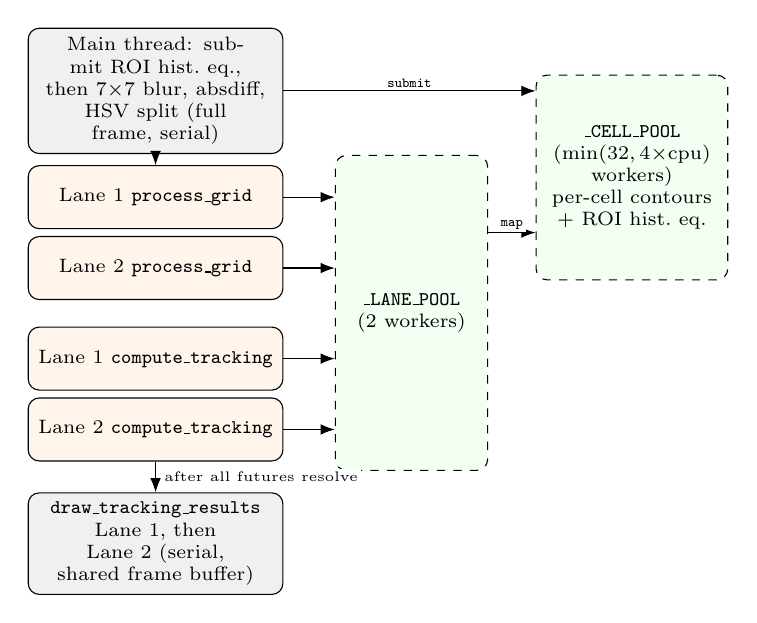
\begin{tikzpicture}[
  box/.style={draw, rounded corners, align=center, minimum height=0.8cm,
              text width=3.0cm, font=\scriptsize, fill=orange!8},
  serial/.style={box, fill=gray!12},
  pool/.style={draw, dashed, rounded corners, align=center, font=\scriptsize,
               fill=green!5, text width=1.7cm},
  arr/.style={-{Latex[length=1.8mm]}},
  lbl/.style={font=\tiny, fill=white, inner sep=1pt}
]
\node[serial] (pre)   at (0, 0)    {Main thread: submit ROI hist.\ eq.,\\then $7{\times}7$ blur, absdiff,\\HSV split (full frame, serial)};
\node[box]    (l1)    at (0,-1.35) {Lane 1 \code{process\_grid}};
\node[box]    (l2)    at (0,-2.25) {Lane 2 \code{process\_grid}};
\node[box]    (t1)    at (0,-3.40) {Lane 1 \code{compute\_tracking}};
\node[box]    (t2)    at (0,-4.30) {Lane 2 \code{compute\_tracking}};
\node[serial] (draw)  at (0,-5.75) {\code{draw\_tracking\_results}\\Lane 1, then Lane 2 (serial,\\shared frame buffer)};
\node[pool, minimum height=4.0cm] (lanepool) at (3.25,-2.82) {\code{\_LANE\_POOL}\\(2 workers)};
\node[pool, minimum height=2.6cm, text width=2.2cm] (cellpool) at (6.05,-1.10) {\code{\_CELL\_POOL}\\($\min(32,4{\times}\text{cpu})$\\workers)\\per-cell contours\\+ ROI hist.\ eq.};
\foreach \n in {l1,l2,t1,t2} \draw[arr] (\n.east) -- (\n.east -| lanepool.west);
\draw[arr] (pre.east) -- node[lbl, above]{\code{submit}} (pre.east -| cellpool.west);
\draw[arr] (lanepool.east |- l1.east) ++(0,-0.45) coordinate (a) -- node[lbl, above]{\code{map}} (a -| cellpool.west);
\draw[arr] (pre.south) -- (l1.north);
\draw[arr] (t2.south) -- node[lbl, right, xshift=2pt]{after all futures resolve} (draw.north);
\end{tikzpicture}%
}%
\caption{Per-frame dispatch in the two-lane parallel implementation.}
\label{fig:threadpools}
\end{figure}


\subsection{Evaluation}
\label{sec:eval}
UA-DETRAC XML boxes overlapping the ROI are mapped to \{Car, Van, Bus,
Unknown\}. At grid level, each box center labels a cell, giving a
$4\times4$ confusion matrix over \{Empty, Car, Van, Bus\}. At vehicle
level, each scored track is matched to the highest-IoU box ($>0.1$); the
majority label per ground-truth ID fills a $3\times3$ Car/Van/Bus matrix,
from which precision, recall and F1 are computed with a small
$\epsilon$. Predictions at frame $t$ are compared with ground truth at
$t{+}1$, ``others'' matched to a track count as Car, ignored regions are
not masked, and matching is greedy; these choices affect both implementations
equally.

\textbf{Counting ground truth.} The number of annotated vehicles is not a
count of line crossings, so crossing events are derived from the
annotated trajectories: for each UA-DETRAC target, the centre of its box
in consecutive annotated frames; an event is recorded when the centre
crosses the counting line ($y=272$), with direction \emph{down}
(previous $y<272\le$ current $y$) or \emph{up}, and is assigned to the
ROI whose $x$-range contains the centre (events in the 12\,px gap between
the ROIs are excluded). Predicted events are the counter's own events,
replayed from per-frame logs; the replay reproduces the reported per-lane
totals in every run. Predicted events inside UA-DETRAC ignored regions
are excluded. A predicted and a ground-truth event match if
$|\Delta t|\le25$ frames (1\,s) and $|\Delta x|\le80$\,px and the
ground-truth event is downward; matching is one-to-one and greedy by
$|\Delta t|/25+|\Delta x|/80$, with a bonus when the counted track's box
overlaps the same annotated vehicle. An unmatched prediction is a
\emph{duplicate} if its vehicle, or a compatible ground-truth event, was
already matched, and a \emph{false count} otherwise; unmatched downward
events are \emph{missed counts}, and upward events are \emph{directional
omissions}. In the combined score both ROIs compete for one list of
ground-truth events, so a vehicle is never credited twice. We report
event precision $TP/P$, recall $TP/G$, $F_1=2TP/(P+G)$ and, per video,
the count error $P-G$ as MAE, RMSE and MAPE (videos with $G>0$).

\textbf{Statistics.} Grid comparisons on the test set are paired (all grids
run on the same videos). The resampling unit is the camera site (12
groups); we report 95\% percentile bootstrap intervals (4000 resamples)
and two-sided paired permutation tests that swap the two grids' results
within randomly chosen sites. For each metric, the three comparisons
against $6{\times}6$ are Holm-adjusted; we also report the correction
over all 18 tests.

\section{Experimental Setup}
\label{sec:experiments}
\textbf{Platform.} AMD Ryzen 5 7235HS laptop (4 cores, 8 logical
processors), Windows 11, Python 3.12.3, OpenCV 4.12.0, NumPy 1.26.4;
each metrics file records these values \cite{beyer2019}.

\textbf{Videos.} From each UA-DETRAC weather folder (Cloudy, Night,
Rainy, Sunny) we split the annotated videos into density terciles (mean
annotated vehicles per frame) and took the middle-ranked video of each,
giving 12 videos (2.81--14.92 vehicles/frame; 960$\times$540, 25\,fps;
14{,}356 frame pairs). Tiers are relative within each category; the
candidate pools were small (4/6/5/23 videos). Grid $6\times6$, channel V,
display and frame dumps disabled.

\textbf{Four workloads.} The sequential implementation processes one
ROI and the two-lane parallel implementation two, so their raw times are
not comparable. We therefore time: \textbf{A}~\code{seq.py} (1 lane);
\textbf{B}~the parallel implementation with Lane~1 only (threaded);
\textbf{C}~both lanes with the thread pools replaced by an inline executor
(same \code{LaneTracker} code and call order, no threads: the unthreaded
workload); and \textbf{D}~the parallel implementation (2 lanes, threaded). With end-to-end time $T$ and mean per-frame
processing time $\bar t$ (processing and drawing, excluding output I/O,
same boundaries in all workloads) we report per video
$S_{\text{naive}}=T_A/T_D$ (context only), the ROI-frame throughput ratio
$S_{\text{norm}}=2T_A/T_D$, its unthreaded counterpart
$S_{\text{amort}}=2T_A/T_C$, and the threads-only ratios
$S_{\text{same}}^{(2)}=T_C/T_D$ and $S_{\text{same}}^{(1)}=T_A/T_B$.
Because decoding, writing and the full-frame preprocessing are done once
per frame, $S_{\text{norm}}$ can exceed 1 without any benefit from
threading. Values are mean $\pm$ sample std over the 12 videos, i.e.\
between-video variation. Each workload ran once per video with the
profiler off; A and D were also run under \code{cProfile}. All numbers
are computed by \code{benchmarking/orchestrate\_benchmark.py}.

\textbf{Grid-resolution study.} Six resolutions ($4{\times}6$ to
$10{\times}12$, rows$\times$columns) were run on workload~C (both lanes,
no threads) on a separate 2-vCPU Linux VM (OpenCV~5.0); its frame rates
are not comparable with the benchmark machine. UA-DETRAC has no
camera-site labels, so sites were inferred from median-background
thumbnails of all 100 videos (road layout, medians, fences, buildings
and street furniture), cross-checked by an automatic gradient-correlation
clustering; doubtful pairs were merged, because over-merging only reduces
the number of folds whereas under-merging leaks scene information. The
26 annotated videos of the four weather folders that are not benchmark
videos (30{,}427 frames, 10 site groups) were used for selection only.
The test set is 44 further videos (67{,}206 frames, 12 site groups) that
no earlier experiment used and whose scenes resemble none of the 38
tuning and benchmark videos; 18 resembling videos were excluded. The
12 benchmark videos share sites with the tuning videos (8 of 12) and had
informed an exploratory analysis, so they are not used for grid
comparisons. The complete video-to-site mapping, with the uncertain
assignments, is supplementary material.

Selection used leave-one-site-out cross-validation on the 26 videos. In
each fold and for each grid $g$, the thresholds $\theta_g$ were chosen
from 810 candidate rules (Bus/Van span thresholds, optionally a Van
aspect limit) to maximise pooled macro-F1 on the training sites. Grids
were then scored by
\begin{equation}
\begin{split}
J(g)={}&0.30\,F_1^{\text{mac}}+0.10\,\min_c F_1^{c}+0.25\,F_1^{\text{cnt}}\\
&+0.15\,R^{\text{det}}+0.10\,(1-\phi)+0.10\,(1-u),
\end{split}
\label{eq:objective}
\end{equation}
where all terms lie in $[0,1]$, are pooled over the scored videos and are
not further normalized: $F_1^{\text{mac}}$ and $F_1^{c}$ are vehicle-level
macro and per-class F1 with $\theta_g$, $F_1^{\text{cnt}}$ is the combined
counting event-F1 against downward crossings, $R^{\text{det}}$ is the
fraction of ground-truth vehicles matched by a track, $\phi$ is the
fraction of ground-truth observations covered by two or more detections
(fragmentation), and $u$ is the fraction of predicted tracks matching no
ground-truth vehicle. Only grids with a median of at least 25\,FPS in
three serial timing trials and at most 1.5 times the $6{\times}6$ peak
memory were eligible (all were). Among eligible grids within 0.005 of the
best $J$, the one with the fewest cells was chosen. The weights were set
before any cross-validation or test result was computed and were not
changed afterwards; the frozen configuration was recorded before the
test set was assembled.

\section{Results and Discussion}
\label{sec:results}

\subsection{Accuracy and Cross-Implementation Equivalence}
\label{sec:crosscheck}
Because \code{seq.py} and Lane~1 of the parallel implementation run the
same deterministic logic on the same ROI, their confusion matrices should
agree exactly. Initially only 4 of 12 videos matched. The parallel
version lacked the $7\times7$ pre-difference blur; adding it raised the
match rate only to 5/12. The remaining divergence was in the
equalization itself: the parallel helper ignored the channel setting and
grayscaled the ROI, discarding hue and saturation, whereas \code{seq.py}
equalizes only V. (The pre-fix runs were not archived; both match rates
are taken from development logs.) After both fixes, Lane~1 of
workloads B, C and D matches \code{seq.py} on all 12 videos
(vehicle and grid matrices, ID counts and per-class P/R/F1, compared
exactly), and Lane~2 matches between C and D: 60/60 checks, including the
profiled pass. This shows agreement on the tested videos under this
protocol, not equivalence for every input.

Table~\ref{tab:prf} reports the resulting
vehicle-level metrics, computed per video and averaged as elsewhere in
the paper. Accuracy is low and varies strongly between videos. Pooled
over the 12 videos, 179 of the 203 matched ground-truth vehicles are
cars, but the classifier labels 127 of them as vans; this systematic
Car$\to$Van bias of the fixed geometric thresholds explains the low Car
recall and the low Van precision. Vans and buses occur in the matched
ground truth of only 7 and 5 videos, and a class that is absent or never
reaches the minimum track age scores 0 for that video, so Bus F1 is 0 in
10 of 12 videos and in four of seven groups. The contribution of this
section is the verified agreement between implementations, not the
classifier's accuracy.

\begin{table}[t]
\centering
\caption{Vehicle-level precision, recall and F1 (identical for both
implementations), mean $\pm$ std over 12 videos.}
\label{tab:prf}
\scriptsize
\setlength{\tabcolsep}{4pt}
\begin{tabular}{lcccc}
\toprule
\textbf{Class} & \textbf{Precision} & \textbf{Recall} & \textbf{F1} & \textbf{Videos with class$^{a}$} \\
\midrule
Car & $0.51\pm0.46$ & $0.24\pm0.32$ & $0.29\pm0.31$ & 12 \\
Van & $0.07\pm0.11$ & $0.33\pm0.45$ & $0.11\pm0.16$ & 7 \\
Bus & $0.03\pm0.08$ & $0.10\pm0.23$ & $0.04\pm0.12$ & 5 \\
\bottomrule
\end{tabular}

\smallskip
\parbox{\columnwidth}{\scriptsize $^{a}$Videos whose matched ground truth
contains the class; in the other videos the class scores 0.}
\end{table}

\subsection{Grid Resolution Sensitivity and Its Impact on Vehicle Classification and Counting}
\label{sec:grid-sensitivity}
\textbf{Selection.} Out-of-fold $J$ ranged only from 0.518 to 0.538 across
the six grids, and the per-fold rule chose $6{\times}8$ in 8 of 10 folds.
On all 26 tuning videos, $J$ was 0.546 ($8{\times}8$), 0.543
($10{\times}12$), 0.543 ($6{\times}8$) and 0.537 ($6{\times}6$), so the tie
rule selected $6{\times}8$ with thresholds Bus if column span $>0.90$ or
both spans $>0.75$, Van if row span $>0.70$ and box aspect $\le2.5$. This
margin is smaller than the fold-to-fold variation; the choice is
reproducible from Eq.~\eqref{eq:objective}, not evidence that
$6{\times}8$ is generally best.

\begin{table}[t]
\centering
\caption{Grid resolution on the 44 unseen-site test videos (per-grid tuned
thresholds; combined lanes). Det.\ rec.: matched ground-truth vehicles;
Frag.: fragmentation; count metrics use downward crossings. FPS: median
of 3 serial trials on the VM. $^{\dagger}$Differs from $6{\times}6$ after
Holm adjustment within the metric ($p<0.05$).}
\label{tab:grid}
\scriptsize
\setlength{\tabcolsep}{2.4pt}
\begin{tabular}{lcccccccc}
\toprule
\textbf{Grid} & \textbf{Mac.-F1} & \textbf{W.-F1} & \textbf{Det.\ rec.} & \textbf{Frag.} & \textbf{Cnt.\ F1} & \textbf{MAE} & \textbf{RMSE} & \textbf{FPS}\\
\midrule
$6{\times}6$     & 0.405 & 0.782 & 0.882 & 1.5\% & 0.314 & 16.0 & 20.4 & 97.2\\
$6{\times}8^{a}$ & 0.416 & 0.799 & 0.892 & 2.3\% & 0.336$^{\dagger}$ & 14.9 & 18.5 & 91.9\\
$8{\times}8$     & 0.402 & 0.813 & 0.894 & 3.8\% & 0.342 & 16.6 & 20.3 & 86.3\\
$10{\times}12$   & 0.430 & 0.815 & 0.908 & 9.5\% & 0.337 & 23.1$^{\dagger}$ & 26.6$^{\dagger}$ & 81.4\\
always-Car       & 0.310 & 0.805 & -- & -- & -- & -- & -- & --\\
\bottomrule
\end{tabular}

\smallskip
\parbox{\columnwidth}{\scriptsize $^{a}$Selected configuration. Always-Car
values vary by $\le0.004$ across grids (row shows $6{\times}8$).}
\end{table}

\begin{table}[t]
\centering
\caption{Test-set classification of the selected $6{\times}8$
configuration (vehicle level, pooled over 44 videos).}
\label{tab:cls}
\scriptsize
\setlength{\tabcolsep}{3.2pt}
\begin{tabular}{lccccccc}
\toprule
\textbf{True} & \multicolumn{3}{c}{\textbf{Predicted}} & \textbf{$n$} & \textbf{Prec.} & \textbf{Rec.} & \textbf{F1}\\
\cmidrule(lr){2-4}
 & Car & Van & Bus & & & & \\
\midrule
Car & 1472 & 126 & 34 & 1632 & 0.889 & 0.902 & 0.895\\
Van & 112 & 23 & 2 & 137 & 0.132 & 0.168 & 0.148\\
Bus & 72 & 25 & 17 & 114 & 0.321 & 0.149 & 0.204\\
\bottomrule
\end{tabular}

\smallskip
\parbox{\columnwidth}{\scriptsize Macro-F1 0.416 vs.\ 0.310 for
always-Car (difference 95\% CI $[0.060, 0.152]$); weighted-F1 0.799 vs.\
0.805 (CI $[-0.022, 0.022]$); accuracy 0.803 vs.\ 0.867. Car$\to$Van
7.7\%, Van$\to$Car 81.8\%, Bus$\to$Car 63.2\%.}
\end{table}

\begin{table*}[t]
\centering
\caption{Counting on the 44 test videos by lane (downward-crossing ground truth; $G_{\uparrow}$:
upward events, never countable). False: unmatched predictions (in brackets: caused by
upward-moving vehicles); Missed: unmatched downward events (in brackets: vehicle not detected
near the line). In the combined scope both ROIs compete for one ground-truth list, so its
TP can exceed the sum of the lanes when a vehicle is counted in the neighbouring ROI.}
\label{tab:count}
\scriptsize
\setlength{\tabcolsep}{3.4pt}
\begin{tabular}{llrrrrrrrcccrr}
\toprule
\textbf{Grid} & \textbf{Scope} & $G_{\downarrow}$ & $G_{\uparrow}$ & $P$ & \textbf{TP} & \textbf{False} & \textbf{Dup.} & \textbf{Missed} & \textbf{Prec.} & \textbf{Rec.} & \textbf{F1} & \textbf{MAE} & \textbf{RMSE}\\
\midrule
$6{\times}6$ & Lane 1 & 501 & 126 & 766 & 217 & 524 (35) & 25 & 284 (14) & 0.283 & 0.433 & 0.343 & 11.4 & 15.0\\
 & Lane 2 & 219 & 434 & 611 & 104 & 483 (125) & 24 & 115 (4) & 0.170 & 0.475 & 0.251 & 10.4 & 14.0\\
 & Combined & 720 & 560 & 1377 & 329 & 974 (172) & 74 & 391 (18) & 0.239 & 0.457 & 0.314 & 16.0 & 20.4\\
\midrule
$6{\times}8$ & Lane 1 & 501 & 126 & 714 & 229 & 464 (35) & 21 & 272 (11) & 0.321 & 0.457 & 0.377 & 10.3 & 13.2\\
 & Lane 2 & 219 & 434 & 604 & 104 & 487 (141) & 13 & 115 (2) & 0.172 & 0.475 & 0.253 & 10.3 & 13.6\\
 & Combined & 720 & 560 & 1318 & 342 & 915 (182) & 61 & 378 (13) & 0.259 & 0.475 & 0.336 & 14.9 & 18.5\\
\midrule
$8{\times}8$ & Lane 1 & 501 & 126 & 765 & 251 & 494 (43) & 20 & 250 (20) & 0.328 & 0.501 & 0.397 & 10.5 & 13.7\\
 & Lane 2 & 219 & 434 & 663 & 107 & 539 (154) & 17 & 112 (3) & 0.161 & 0.489 & 0.243 & 11.4 & 14.9\\
 & Combined & 720 & 560 & 1428 & 367 & 1007 (212) & 54 & 353 (23) & 0.257 & 0.510 & 0.342 & 16.6 & 20.3\\
\midrule
$10{\times}12$ & Lane 1 & 501 & 126 & 931 & 282 & 613 (54) & 36 & 219 (19) & 0.303 & 0.563 & 0.394 & 12.9 & 16.1\\
 & Lane 2 & 219 & 434 & 797 & 125 & 632 (171) & 40 & 94 (2) & 0.157 & 0.571 & 0.246 & 13.9 & 17.8\\
 & Combined & 720 & 560 & 1728 & 413 & 1219 (238) & 96 & 307 (21) & 0.239 & 0.574 & 0.337 & 23.1 & 26.6\\
\bottomrule
\end{tabular}
\end{table*}

\begin{figure}[t]
\centering
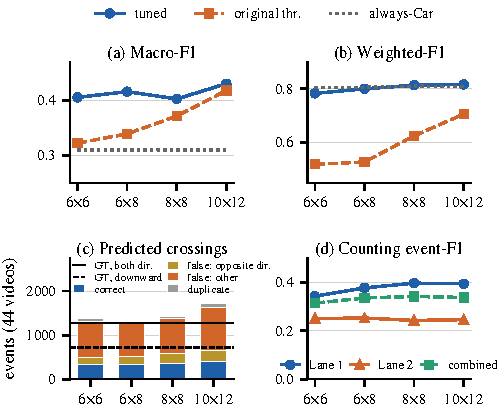
\includegraphics[width=\columnwidth]{figures/fig_grid.pdf}
\caption{Grid resolution on the 44 unseen-site test videos.
(a)~Macro-F1 and (b)~weighted-F1 with the original and the per-grid tuned
thresholds, against always-Car. (c)~Predicted crossings by outcome,
combined lanes, against downward and all trajectory crossings.
(d)~Counting event-F1 per lane.}
\label{fig:grid}
\end{figure}

\textbf{Classification.} With the original thresholds, test macro-F1 rose
with resolution from 0.322 to 0.418 (Fig.~\ref{fig:grid}a); after per-grid
tuning it was 0.402--0.430 for every grid (Table~\ref{tab:grid}), and no
grid differed from $6{\times}6$ (differences $\le0.025$, Holm-adjusted
$p=1.0$). The earlier resolution trend was therefore a calibration effect
of fixed normalized-span thresholds. The tuned classifier beats always-Car
in macro-F1, but its weighted-F1 (0.78--0.82) and accuracy are not higher
(Table~\ref{tab:cls}): it labels 82\% of vans and 63\% of buses as cars
(Van recall 0.17, Bus recall 0.15) and is not a reliable three-class
classifier.

\textbf{Counting.} Table~\ref{tab:count} separates the error sources.
\emph{Directional omissions}: 560 of the 1{,}280 test crossings (44\%)
are upward; 434 of them occur in Lane~2, where upward traffic dominates
(as in the tuning videos: 457 of 739), so the counter never counts that
lane's main direction. \emph{False counts} are the largest error
(915--1{,}219); 18--21\% come from upward-moving vehicles whose cluster
centroid jumps downward across the line, and at $6{\times}8$, 701 of the
976 unmatched predictions overlap no annotated vehicle (spurious motion
clusters). \emph{Missed downward counts} are mostly association failures:
at $6{\times}8$, 365 of 378 missed vehicles were detected near the line,
but no track crossed it (for example because the track started below the
line or was split). \emph{Duplicates} (54--96) are highest at
$10{\times}12$. Track association is weak at every resolution: a
ground-truth vehicle is covered by 2.5--3.1 tracks on average, and
69--75\% of vehicles have at least one identity switch.

With finer grids, correct counts rise (329 to 413) but false and
duplicate counts rise faster (1{,}048 to 1{,}315), so the per-video
error grows at $10{\times}12$: MAE $+7.1$ (95\% CI $[5.4, 8.4]$,
Holm-adjusted $p=0.010$) and RMSE $+6.2$ ($p=0.013$) relative to
$6{\times}6$. $6{\times}8$ raises counting F1 by 0.022 ($[0.012, 0.030]$,
$p=0.012$), a statistically supported but small gain. Its objective gain
($J$: $+0.011$, nominal $p=0.03$) does not survive the Holm adjustment
($p=0.09$), and $10{\times}12$ does not change $J$ ($+0.0004$, $p=0.96$).
Corrected over all 18 tests, no difference reaches $p<0.05$ (smallest:
$10{\times}12$ MAE, $p=0.058$). In practical terms, the macro-F1
differences are small, while 7 extra count errors per video at
$10{\times}12$ (+44\%) are large.

\textbf{Why fragmentation grows.} After the per-cell dilation, a single
pixel above threshold fills its cell, so the 100\,px$^2$ contour filter
never takes effect. As cells shrink (from $73{\times}23$ to
$36{\times}14$\,px), the interiors of vehicles, which frame differencing
leaves unmarked, become empty cells that split a vehicle into several
clusters. In separately run diagnostic variants on the tuning videos,
bridging a single empty cell row removed 87--89\% of the fragmentation and
8-connectivity removed 35--40\%. Neither improved classification.

\subsection{Timing: Four Workloads}
\label{sec:timing}

\begin{table}[t]
\centering
\caption{Four workloads (clean pass), mean $\pm$ std over 12 videos.}
\label{tab:timing}
\scriptsize
\setlength{\tabcolsep}{2.5pt}
\begin{tabular}{lcccccc}
\toprule
 & \textbf{Ln.} & \textbf{Loop (ms)} & \textbf{I/O (ms)} & \textbf{FPS} & \textbf{Peak MB} & \textbf{CPU} \\
\midrule
A & 1 & $9.41\pm1.84$ & $2.26\pm0.46$ & $81.1\pm15.7$ & $302.5\pm1.9$ & $4.20\pm0.61$ \\
B & 1 & $11.10\pm1.99$ & $2.19\pm0.43$ & $72.0\pm12.2$ & $306.4\pm1.8$ & $4.01\pm0.50$ \\
C & 2 & $14.54\pm2.59$ & $2.09\pm0.36$ & $58.2\pm9.6$ & $306.0\pm3.0$ & $4.52\pm0.47$ \\
D & 2 & $17.46\pm3.73$ & $2.27\pm0.39$ & $50.1\pm9.4$ & $310.0\pm3.1$ & $3.94\pm0.70$ \\
\bottomrule
\end{tabular}

\smallskip
\parbox{\columnwidth}{\scriptsize Loop: per-frame processing and drawing;
I/O: video write and next-frame decode; FPS: video frames per second of
end-to-end time; CPU: process CPU time / wall time (cores).}
\end{table}

\begin{figure}[t]
\centering
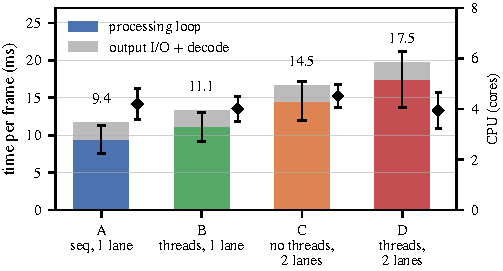
\includegraphics[width=\columnwidth]{figures/fig_workloads.pdf}
\caption{Per-frame time of the four workloads (bars, left axis) and CPU
use in cores (diamonds, right axis); mean $\pm$ std over 12 videos.}
\label{fig:workloads}
\end{figure}

Table~\ref{tab:timing} and Fig.~\ref{fig:workloads} summarize the
timings. Per video:
$S_{\text{naive}}=0.628\pm0.114$, $S_{\text{norm}}=1.257\pm0.228$
(per-frame loop: $1.097\pm0.187$), $S_{\text{amort}}=1.458\pm0.216$,
$S_{\text{same}}^{(2)}=0.860\pm0.077$ (loop: $0.842\pm0.081$) and
$S_{\text{same}}^{(1)}=0.900\pm0.123$. Three findings follow. First, the
two-lane parallel run takes longer than the one-lane sequential run on
every video. Second, \textbf{threading does not reduce execution time on
this machine}: with the workload fixed, the threaded run is slower than
the unthreaded one on all 12 videos with two lanes ($S_{\text{same}}^{(2)}$
0.69--0.93) and on 9 of 12 with one lane. Third, the normalized
throughput gain of D over A ($1.26$) is smaller than that of the
unthreaded run C over A ($1.46$), so it comes from processing two lanes
per decoded and preprocessed frame, not from threading
(Fig.~\ref{fig:ratios}). At the lane-pool width $N=2$ the threads-only
efficiency $S_{\text{same}}^{(2)}/N$ is 0.43; other pool widths were not
measured. The
threaded two-lane workload uses 7.5\,MB (2.5\%) more peak memory
than \code{seq.py}. An earlier run of A and D, with asymmetric timer
boundaries, gave $S_{\text{norm}}=1.261\pm0.084$ and identical accuracy.

\begin{figure}[t]
\centering
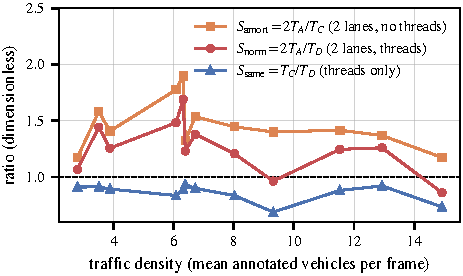
\includegraphics[width=\columnwidth]{figures/fig_ratios.pdf}
\caption{Per-video ratios against traffic density. Two lanes without
threads (C) gain more over the one-lane script than two lanes with
threads (D); threads alone ($T_C/T_D$) are below 1 on every video.}
\label{fig:ratios}
\end{figure}

$S_{\text{norm}}$ correlates weakly and negatively with density
(Pearson $r=-0.45$, $n=12$; heavy tier $1.08\pm0.20$). The cause is
open: tracking takes only 1.6--4.2\% of sequential run time, with no
density trend.

\subsection{Profiling and the Amdahl Ceiling}
\label{sec:results-amdahl}
In the sequential profile of the densest video (MVI\_39311, 1504
frames, 18.62\,s), the seven largest native OpenCV calls (\code{dilate},
\code{GaussianBlur}, \code{VideoCapture.read}, \code{cvtColor},
\code{absdiff}, \code{VideoWriter.write}, \code{split}) take 12.40\,s
(66.6\%), Python wrappers 0.99\,s, the main loop 1.62\,s, and the rest
3.61\,s (1.95\,s in further top-15 native calls such as
\code{findContours}, 0.51\,s). Counting only work reachable through
\code{\_CELL\_POOL} (per-cell contours and equalization) gives $p=0.362$
($0.375\pm0.019$ over all 12 videos); counting the seven native calls
gives $p=0.666$. At the lane-pool width $N=2$, Eq.~\eqref{eq:amdahl}
predicts 1.22 and 1.50 (Fig.~\ref{fig:amdahl}); the measured
threads-only ratio, 0.86, is below 1 and far from both. The narrow ceiling happens to lie close to $S_{\text{norm}}$ (1.22 vs.\
1.26), but the same-workload measurement shows that this proximity is
coincidental: $S_{\text{norm}}$ reflects shared per-frame work, not
threading.

\begin{figure}[t]
\centering
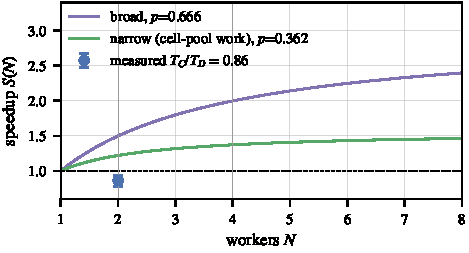
\includegraphics[width=\columnwidth]{figures/fig_amdahl.pdf}
\caption{Amdahl ceilings for the broad and narrow estimates of $p$
(MVI\_39311 profile) and the measured threads-only ratio $T_C/T_D$ at
$N=2$ (mean $\pm$ std).}
\label{fig:amdahl}
\end{figure}

\subsection{Why Threading Does Not Help Here}
\label{sec:why}
For the tested implementation and workloads, Python threading did not
improve performance. This is a measurement of this code on one machine,
not evidence that Python threading is generally slower. Three properties plausibly explain the result; only the first is
measured. (i) \textbf{The cores are already busy}: \code{seq.py} runs one
Python thread but uses $4.20\pm0.61$ cores (Table~\ref{tab:timing})
through native threads inside OpenCV, so Python-level threads compete
for occupied cores; CPU use does not rise with threading (3.94 cores for
D vs.\ 4.52 for C). (ii) \textbf{The tasks are small}: each frame
dispatches 36 tasks per lane on $73\times23$-pixel cells (\code{dilate}
averages $\approx$64\,$\mu$s per call), so dispatch overhead is a large
share of each task. (iii) \textbf{The GIL} serializes the Python parts
(wrappers, clustering, tracking). Separating (ii) and (iii) requires
further experiments, e.g.\ limiting OpenCV's internal threads or
batching cells. The baseline's 26.55\% gain \cite{baseline} was measured
with different code, configuration and hardware, so our results neither
reproduce nor contradict it.

\subsection{Discussion}
\label{sec:discussion}
The grid architecture makes every stage cheap, training-free and
deterministic, which is what allowed exact cross-implementation
agreement and an offline replay of every count. Increasing the resolution
slightly raises detection recall and reduces merging of neighbouring
vehicles, but it also splits vehicles into fragments, which produce extra
tracks and crossing events. Classification with fixed thresholds
therefore favours fine grids, whereas counting favours coarse to medium
ones; after re-tuning, the classification advantage disappears and the
counting cost remains. The geometric features struggle with vans and buses
because the normalized image footprint of a vehicle depends on its
distance from the camera, on occlusion and on fragmentation as much as on
its class, and because vans (7\%) and buses (6\%) are rare among matched
vehicles. Physical dimensions from the calibration, perspective
correction, temporal shape statistics, appearance features and better
association (e.g.\ Kalman filtering with Hungarian matching
\cite{bewley2016,wojke2017}) are the natural next steps; none was
implemented here. The experiments establish the equivalence of the two
implementations on 12 videos, the slowdown from threading on one machine
for this code, and the resolution trade-offs on UA-DETRAC with fixed
ROIs. They do not establish generalization to other cameras or datasets,
the accuracy of the speed estimates, or counting accuracy sufficient for
deployment (test event-F1 $\le0.34$).

\subsection{Threats to Validity}
\label{sec:threats}
All thresholds were tuned for UA-DETRAC geometry, and the two ROIs are
fixed for every video, including intersections in the test set;
illumination, shadows and occlusion remain failure modes
\cite{abbas2021,chen2020}. Camera sites were inferred visually because
UA-DETRAC has no site labels; several merges are uncertain (listed in the
supplementary mapping), and the unseen-site test set still comes from the
same dataset. The weights of Eq.~\eqref{eq:objective} reflect our
judgment and were not optimized. The counter counts only downward
crossings. Speed estimation was not evaluated, uses a single scale without
perspective correction, and produced implausible values in a qualitative
run (Section~\ref{sec:speed}). Benchmark timings come from one laptop and
one run per workload and video; the reported spreads are between-video
variation, and run-to-run variation is visible (sequential loop
$8.03\pm0.29$\,ms in an earlier run vs.\ $9.41\pm1.84$\,ms here), although
the threads-only result has the same sign on all 12 videos. Repeated runs
\cite{kalibera2013} and other machines are needed. The grid study ran on
a different machine and OpenCV version. Tracks younger than 5 frames are
never scored in the classification evaluation.

\section{Conclusion}
\label{sec:conclusion}
We extended a published grid-based detector with classification,
tracking, counting and density estimation (and an unvalidated speed
estimator) in a sequential and a two-lane parallel implementation and
studied it on UA-DETRAC. Measured results: after two preprocessing fixes,
both implementations agree exactly on 12 benchmark videos; on a
4-core/8-thread CPU, the thread pools slowed the same two-lane workload
($0.86\times$), while processing two lanes per decoded frame raised
ROI-frame throughput ($1.46\times$ without threads, $1.26\times$ with
threads); on 44 videos from unseen sites, re-tuned grids from $6{\times}6$
to $10{\times}12$ did not differ in macro-F1, $10{\times}12$ increased the
per-video count error by 44\%, and the tuned classifier did not exceed
always-Car in weighted-F1. Our interpretation is that, for this pipeline,
the footprint features, the single-direction counter and the greedy
association limit accuracy more than the lattice resolution, and that
OpenCV's internal threading leaves little room for Python-level threads.
Future work: direction-aware counting per lane; better association
\cite{bewley2016,wojke2017}; perspective-aware and appearance features
\cite{chang2025,macko2025}; limiting OpenCV's internal threads to test
thread-level parallelism; validated speed estimation \cite{kamil2024};
and repeated benchmarks on several machines. Code, data, metrics and
figure scripts are available in the project repository.


\begin{thebibliography}{99}

\bibitem{baseline}
M. Sankaranarayanan and K. SivaSai, ``Two-tier parallel virtual lattice
layers for enhanced efficiency in video traffic management,''
\emph{Int.\ J. Intell.\ Transp.\ Syst.\ Res.}, vol.~23, no.~1,
pp.~464--474, 2025, doi: 10.1007/s13177-025-00461-4.

\bibitem{muthuraja2026}
S. Muthuraja and M. Sankaranarayanan, ``Real-time traffic density
estimation using scene-adaptive parallel grid analysis,'' Research Square
preprint (in review), Jun.\ 2026, doi: 10.21203/rs.3.rs-9946108/v1.

\bibitem{crouzil2016}
A. Crouzil, L. Khoudour, P. Valiere, and D. N. Truong Cong, ``Automatic
vehicle counting system for traffic monitoring,'' \emph{J. Electron.\
Imaging}, vol.~25, no.~5, art.~051207, 2016, doi:
10.1117/1.JEI.25.5.051207.

\bibitem{lian2025}
H. Lian, M. Li, T. Li, Y. Zhang, Y. Shi, Y. Fan, W. Yang, H. Jiang,
P. Zhou, and H. Wu, ``Vehicle speed measurement method using monocular
cameras,'' \emph{Sci.\ Rep.}, vol.~15, art.~2755, 2025, doi:
10.1038/s41598-025-87077-6.

\bibitem{liu2025}
Y. Liu and S. Shen, ``Vehicle detection and tracking based on improved
YOLOv8,'' \emph{IEEE Access}, vol.~13, pp.~24793--24803, 2025, doi:
10.1109/ACCESS.2025.3538556.

\bibitem{zhai2023}
J. Zhai, B. Li, S. Lv, and Q. Zhou, ``FPGA-based vehicle detection and
tracking accelerator,'' \emph{Sensors}, vol.~23, no.~4, art.~2208, 2023,
doi: 10.3390/s23042208.

\bibitem{chang2025}
L. Chang, Q. Tang, J. Xin, Y. Jiang, H. Zhang, Z. Li, Y. Zhou, and
J. Zhou, ``Low-complexity real-time detection transformer for identifying
bridge vehicle loads,'' \emph{Comput.-Aided Civ.\ Infrastruct.\ Eng.},
vol.~40, no.~26, pp.~4485--4506, 2025, doi: 10.1111/mice.70061.

\bibitem{macko2025}
A. Macko, L. Gajdo\v{s}ech, and V. Kocur, ``Efficient vision-based
vehicle speed estimation,'' \emph{J. Real-Time Image Process.}, vol.~22,
no.~3, art.~123, 2025, doi: 10.1007/s11554-025-01704-z.

\bibitem{unzueta2012}
L. Unzueta, M. Nieto, A. Cort\'es, J. Barandiaran, O. Otaegui, and
P. S\'anchez, ``Adaptive multicue background subtraction for robust
vehicle counting and classification,'' \emph{IEEE Trans.\ Intell.\
Transp.\ Syst.}, vol.~13, no.~2, pp.~527--540, 2012, doi:
10.1109/TITS.2011.2174358.

\bibitem{abbas2021}
A. F. Abbas, U. U. Sheikh, F. T. AL-Dhief, and M. N. H. Mohd, ``A
comprehensive review of vehicle detection using computer vision,''
\emph{TELKOMNIKA}, vol.~19, no.~3, p.~838, 2021, doi:
10.12928/telkomnika.v19i3.12880.

\bibitem{chen2020}
Y. Chen and W. Hu, ``Robust vehicle detection and counting algorithm
adapted to complex traffic environments with sudden illumination changes
and shadows,'' \emph{Sensors}, vol.~20, no.~9, art.~2686, 2020, doi:
10.3390/s20092686.

\bibitem{cheung2004}
S.-C.\ S.\ Cheung and C.\ Kamath, ``Robust techniques for background
subtraction in urban traffic video,'' in \emph{Proc.\ SPIE Visual
Commun.\ Image Process.}, vol.\ 5308, 2004, pp.\ 881--892, doi:
10.1117/12.526886.

\bibitem{suzuki1985}
S.\ Suzuki and K.\ Abe, ``Topological structural analysis of digitized
binary images by border following,'' \emph{Comput.\ Vis.\ Graph.\ Image
Process.}, vol.\ 30, no.\ 1, pp.\ 32--46, 1985, doi:
10.1016/0734-189X(85)90016-7.

\bibitem{bewley2016}
A. Bewley, Z. Ge, L. Ott, F. Ramos, and B. Upcroft, ``Simple online and
realtime tracking,'' in \emph{Proc.\ IEEE Int.\ Conf.\ Image Process.\
(ICIP)}, 2016, pp.~3464--3468, doi: 10.1109/ICIP.2016.7533003.

\bibitem{wojke2017}
N. Wojke, A. Bewley, and D. Paulus, ``Simple online and realtime
tracking with a deep association metric,'' in \emph{Proc.\ IEEE Int.\
Conf.\ Image Process.\ (ICIP)}, 2017, pp.~3645--3649, doi:
10.1109/ICIP.2017.8296962.

\bibitem{kamil2024}
D. A. Kamil, Wahyono, A. Harjoko, and K.-H. Jo, ``Vehicle speed
estimation using consecutive frame approaches and deep image homography
for image rectification on monocular videos,'' \emph{IEEE Access},
vol.~12, pp.~181937--181952, 2024, doi: 10.1109/ACCESS.2024.3508135.

\bibitem{sangsuwan2024}
K. Sangsuwan and M. Ekpanyapong, ``Video-based vehicle speed estimation
using speed measurement metrics,'' \emph{IEEE Access}, vol.~12,
pp.~4845--4858, 2024, doi: 10.1109/ACCESS.2024.3350381.

\bibitem{wen2020}
L.\ Wen, D.\ Du, Z.\ Cai, Z.\ Lei, M.-C.\ Chang, H.\ Qi, J.\ Lim,
M.-H.\ Yang, and S.\ Lyu, ``UA-DETRAC: A new benchmark and protocol for
multi-object detection and tracking,'' \emph{Comput.\ Vis.\ Image
Underst.}, vol.\ 193, art.\ 102907, 2020, doi:
10.1016/j.cviu.2020.102907.

\bibitem{amdahl1967}
G. M. Amdahl, ``Validity of the single-processor approach to achieving
large-scale computing capabilities,'' in \emph{Proc.\ AFIPS Spring Joint
Computer Conf.}, vol.\ 30, 1967, pp.\ 483--485, doi:
10.1145/1465482.1465560.

\bibitem{alhayanni2020}
M. A. N. Al-hayanni, F. Xia, A. Rafiev, A. Romanovsky, R. Shafik, and
A. Yakovlev, ``Amdahl's law in the context of heterogeneous many-core
systems -- a survey,'' \emph{IET Comput.\ Digit.\ Tech.}, vol.~14,
no.~4, pp.~133--148, 2020, doi: 10.1049/iet-cdt.2018.5220.

\bibitem{poolla2023}
C. Poolla and R. Saxena, ``On extending Amdahl's law to learn computer
performance,'' \emph{Microprocess.\ Microsyst.}, vol.~96, art.~104745,
2023, doi: 10.1016/j.micpro.2022.104745.

\bibitem{beyer2019}
D. Beyer, S. L\"owe, and P. Wendler, ``Reliable benchmarking:
requirements and solutions,'' \emph{Int.\ J. Softw.\ Tools Technol.\
Transf.}, vol.~21, no.~1, pp.~1--29, 2019, doi:
10.1007/s10009-017-0469-y.

\bibitem{kalibera2013}
T. Kalibera and R. Jones, ``Rigorous benchmarking in reasonable time,''
in \emph{Proc.\ Int.\ Symp.\ Memory Management (ISMM)}, 2013,
pp.~63--74, doi: 10.1145/2464157.2464160.

\bibitem{pythongil}
Python Software Foundation, ``Thread states and the global interpreter
lock,'' \emph{Python/C API Reference Manual}. [Online]. Available:
\url{https://docs.python.org/3/c-api/threads.html} (accessed Nov.\ 25, 2026).

\bibitem{pythonfutures}
Python Software Foundation, ``\code{concurrent.futures} --- Launching
parallel tasks,'' \emph{Python 3 documentation}. [Online]. Available:
\url{https://docs.python.org/3/library/concurrent.futures.html}
(accessed Nov.\ 25, 2026).

\end{thebibliography}

\end{document}
